%!TEX root=../../main.tex


\subsubsection{PageRank}
\todo{Einleitung}
In this section we compare the pagerank performance of the various frameworks. As usual we begin with the single-node performance and finish by discussing the distributed variants.

\paragraph{Single-Node}
Ligra and Polymer support both regular and Delta-PageRank variants.
Ligra's regular PR implementation is faster on 4 of 7 graphs. If the regular version is slower than delta, that is only by a small difference. Explicitly, regular is slower than delta by a range of 6\% to 19\%\ on twitter, rMat27 or friendster. For the other graphs, the delta version is slower by a far greater margin of 13\% to 68\%.
Hence, we only show the results of Ligra's regular PageRank implementation in our evaluation.
For Polymer we found the delta version to be faster on all graphs except rMat28. Delta-PR is on average 15\%\ faster on the first six graphs, while only being 0.3\%\ slower on rMat28.
Thus, the following only shows Polymer's faster Delta-PR implementation.
Giraph required more than the available 250 GB of RAM on any graph larger than wikipedia, hence all of Giraph's results for the larger graphs are missing here.
\begin{figure*}
	\hfil
	\begin{subfigure}{0.32\textwidth}
		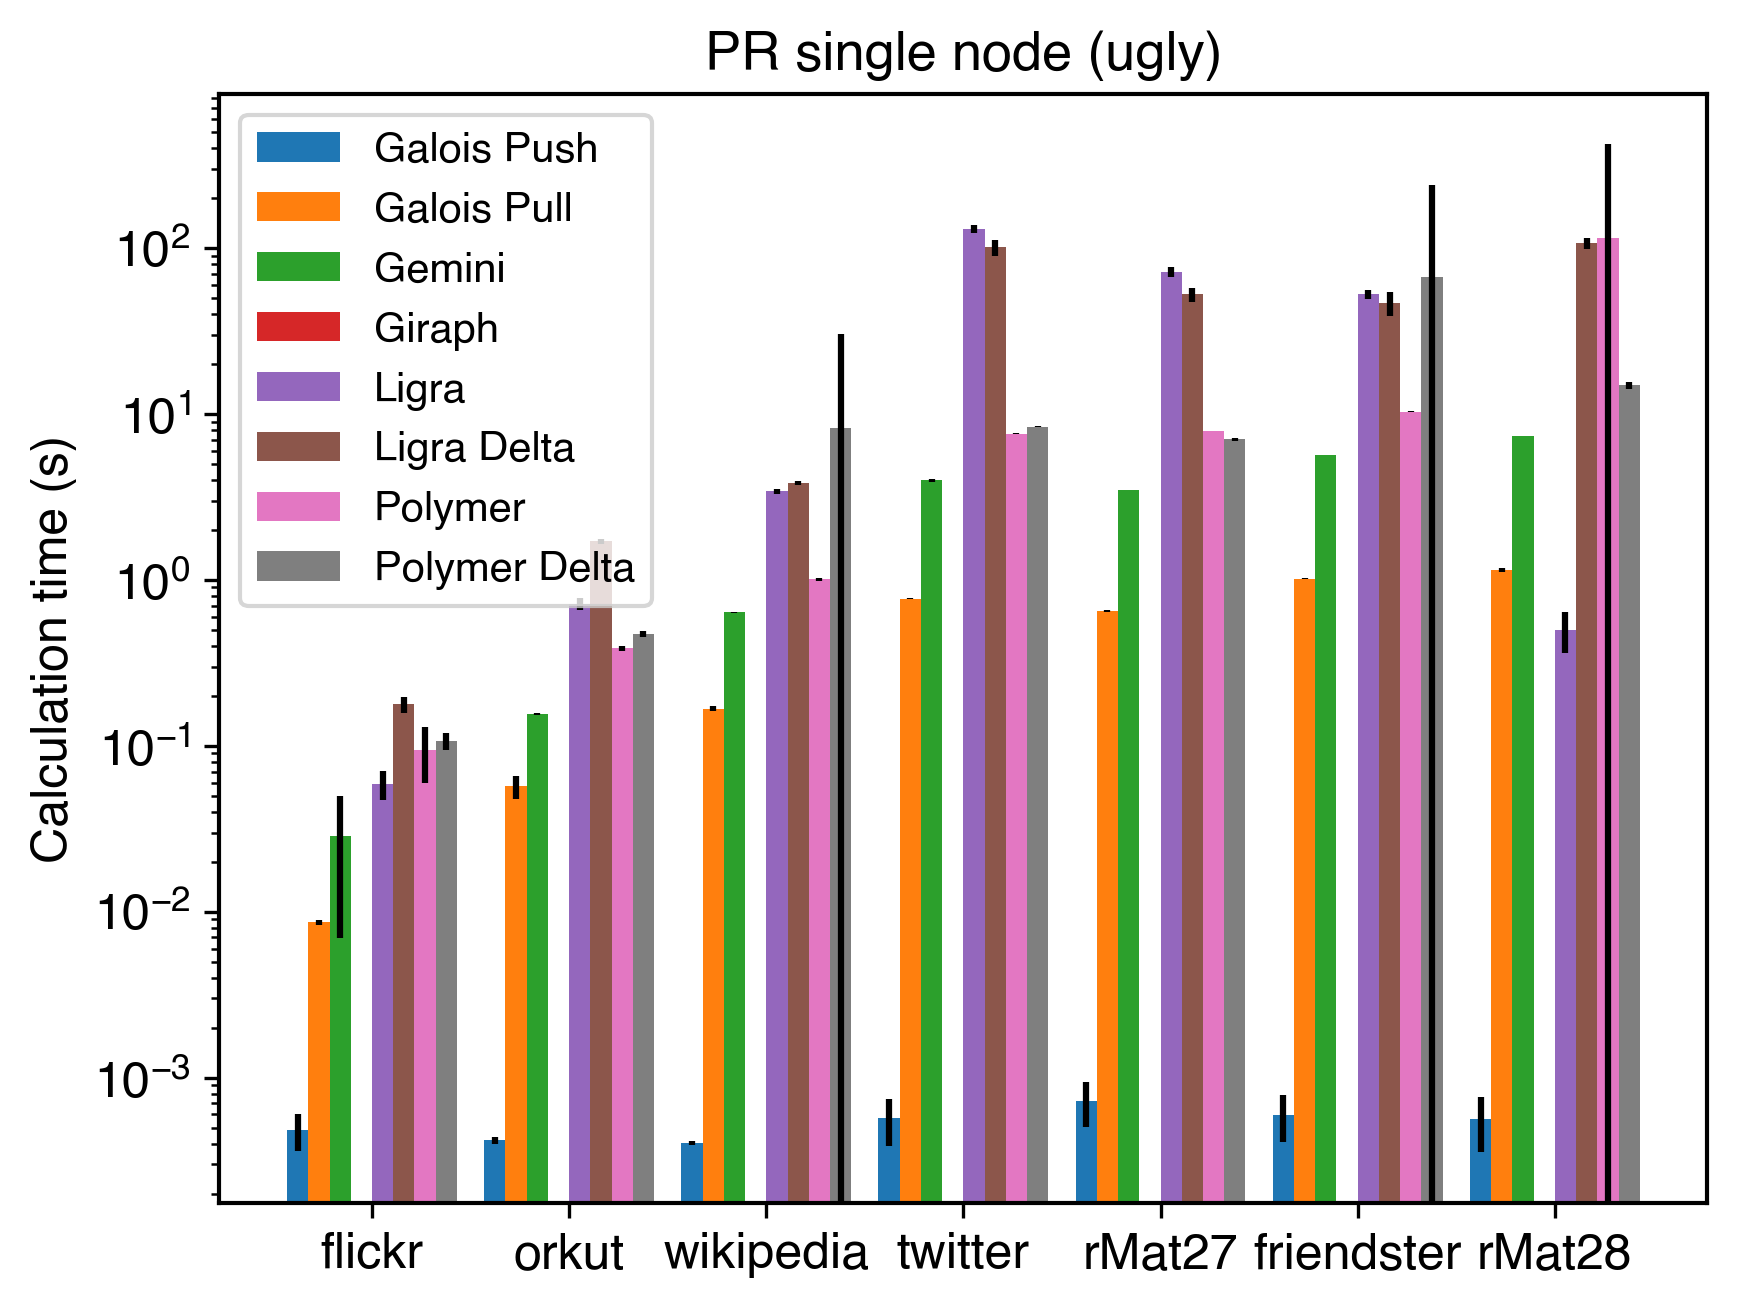
\includegraphics[width=\linewidth]{../../plots/singleNodePR_calcTime.png}
		\caption{Calculation time}
		\label{fig:singleNodePR_calc}
	\end{subfigure}
	\hfil
	\begin{subfigure}{0.32\textwidth}
		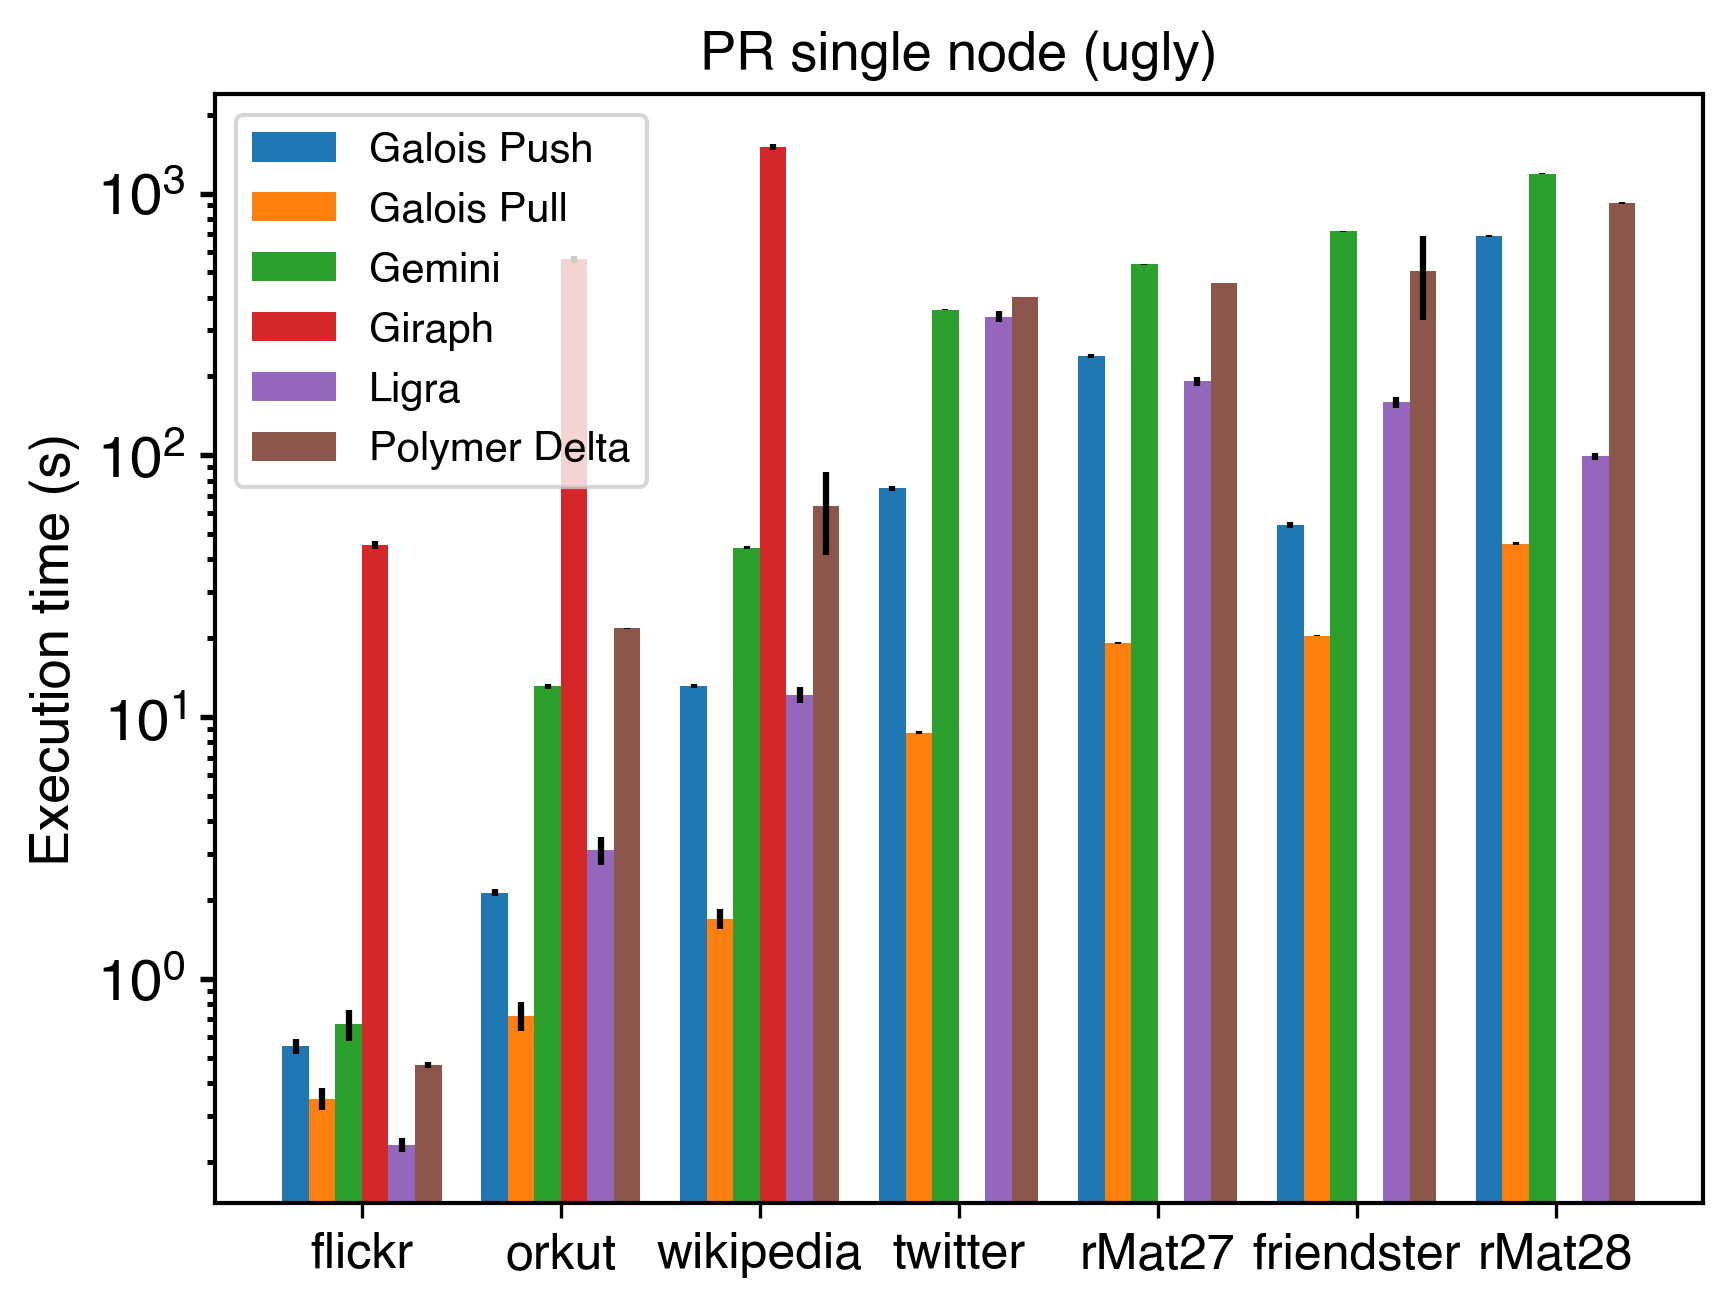
\includegraphics[width=\linewidth]{../../plots/singleNodePR_execTime.png}
		\caption{Execution time}
		\label{fig:singleNodePR_exec}
	\end{subfigure}
	\hfil
	\caption{Average times for PR on a single computation node, black bars represent one standard deviation in our testing}
	\label{fig:singleNodePR}
\end{figure*}

The calculation times show some odd behaviour of Galois Push. The required time is less than 1ms, regardless of the graph (cf. \autoref{fig:singleNodePR_calc}). Meanwhile there was no output produced, that would indicate any kind of error. These results would make the calculation times of Galois Push the smallest on all graphs, with a difference of at least one order of magnitude. However, we are very suspicious of these results and thus exclude the calculation time for Galois Push in further comparisons. Because the execution time of Galois Push is always considerably longer than the execution time of Galois Pull (cf. \autoref{fig:singleNodePR_calc}). This leads us to believe that the output that we used for our measurements contains an error.

For the three graphs on which Giraph computed successfully, it is the slowest framework in both calculation and execution times. And that by a difference of three orders of magnitude in the calculation time and one to two orders of magnitude in execution time (cf \autoref{fig:singleNodePR}). On the larger graphs (i.e. those, where there is no data for Giraph), Gemini and Ligra are always slowest in execution time.
Contrary to this, Galois Pull has the smallest execution times on all graphs except flickr (cf. \autoref{fig:singleNodePR_exec}). Ligra is fastest on flickr, while being second fastest on wikipedia, rMat27 and rMat28. Galois Push is second fastest on orkut and friendster.
Interestingly, the execution time for Ligra is at a maximum for twitter. The required time is steadily decreasing with increasing graph size.



\paragraph{Distributed}
The \autoref{fig:distributedPR} shows our results of PageRank on the distributed cluster.
First of all, Giraph was unable to complete the test because it required more than 250GB of RAM for rMat28, thus this result is missing.
When comparing the calculation times in \autoref{fig:distributedPR_calc} to the execution times in \autoref{fig:distributedPR_exec}, we see similar behaviour of all frameworks. This means that unlike with SSSP or BFS, the calculation times and execution times are similar with respect to the relations of the frameworks to one another. More specifically, there are no overhead outliers like it was the case with Giraph on SSSP.
\begin{figure*}
	\hfil
	\begin{subfigure}{0.32\textwidth}
		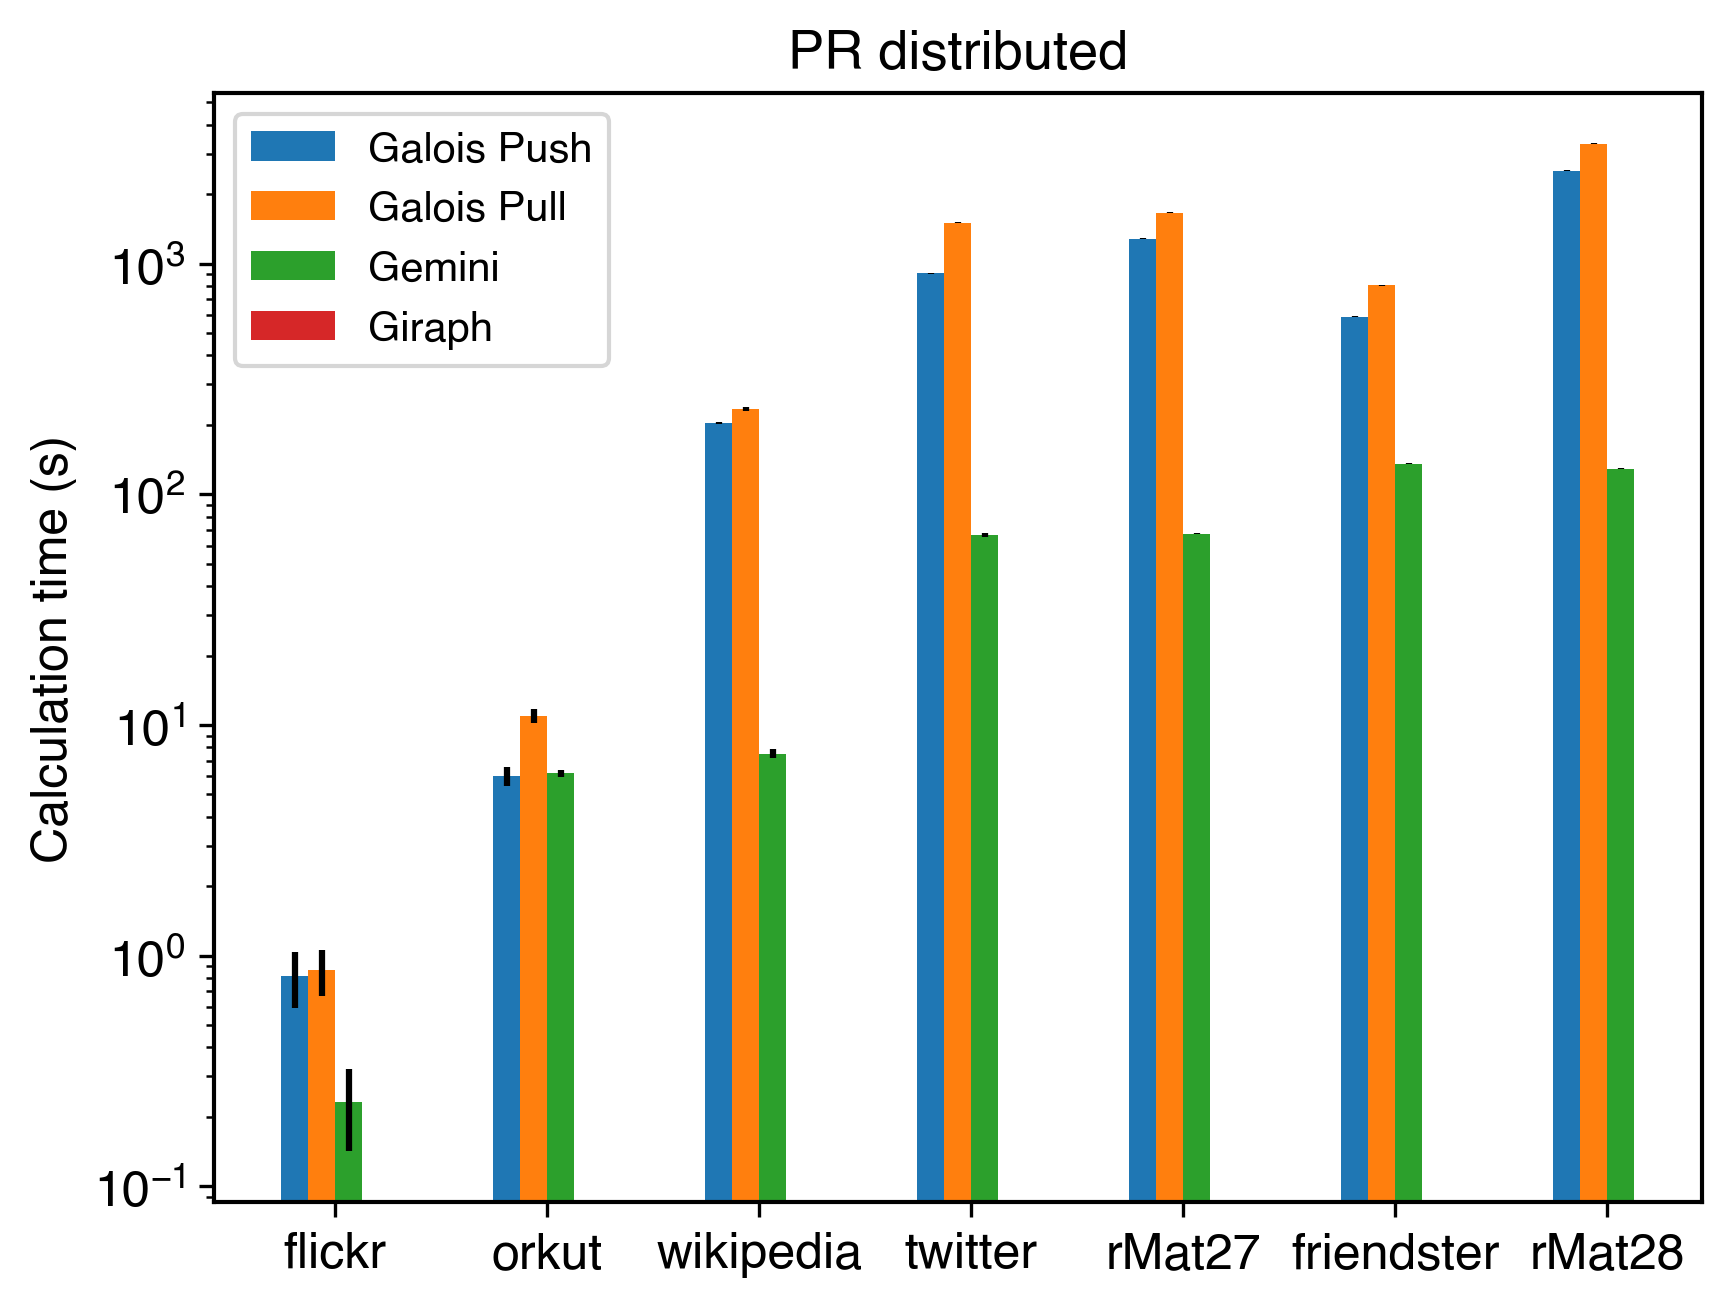
\includegraphics[width=\linewidth]{../../plots/distributedPR_calcTime.png}
		\caption{Calculation time}
		\label{fig:distributedPR_calc}
	\end{subfigure}
	\hfil
	\begin{subfigure}{0.32\textwidth}
		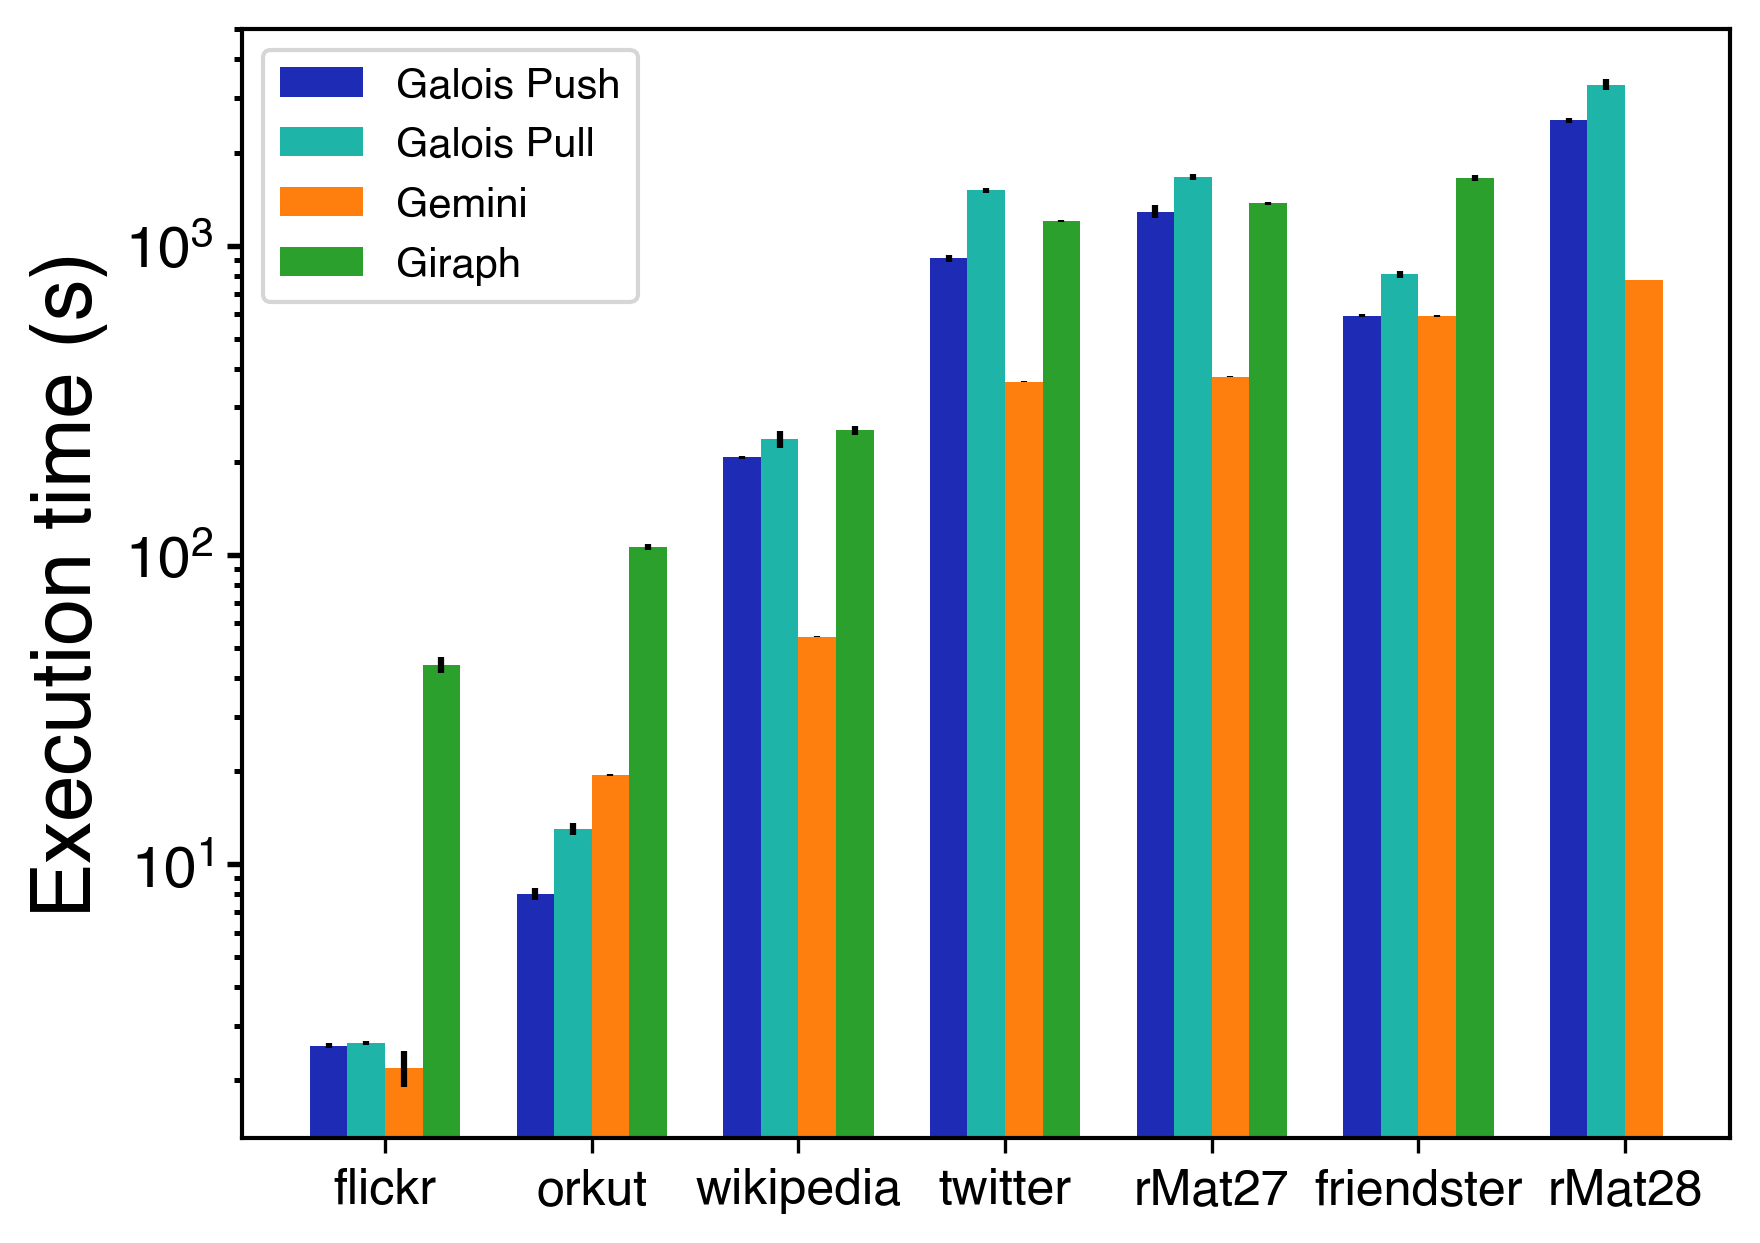
\includegraphics[width=\linewidth]{../../plots/distributedPR_execTime.png}
		\caption{Execution time}
		\label{fig:distributedPR_exec}
	\end{subfigure}
	\hfil
	\caption{Average times for PR on the distributed cluster, black bars represent one standard deviation in our testing}
	\label{fig:distributedPR}
\end{figure*}


\todo{Auswertung fehlt noch.}
\todo{Discussion}









